\section{Successes}
\subsection{BERT}
\begin{frame}[c]{BERT: Bidirectional Encoder Representations}
    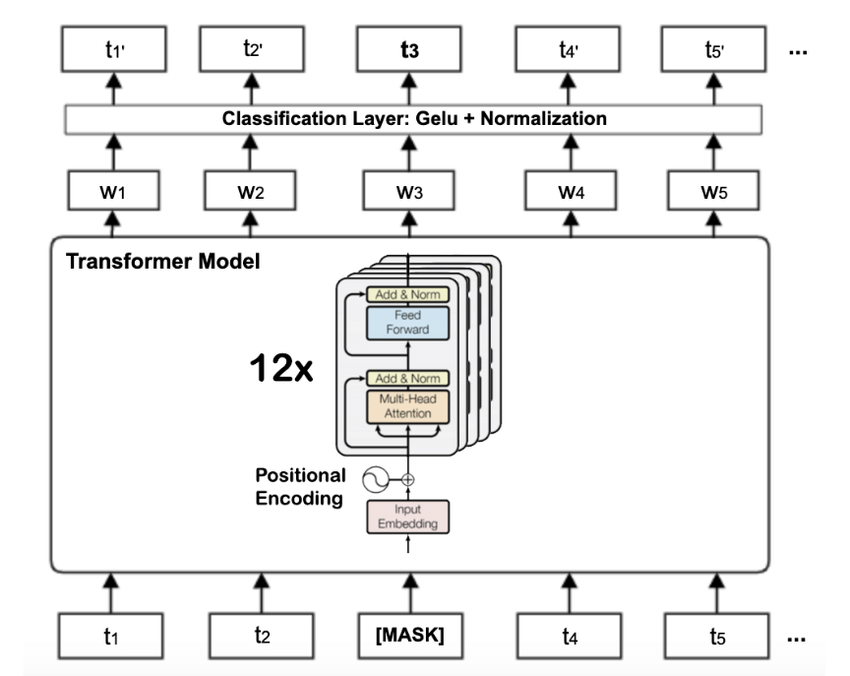
\includegraphics[height=0.8\textheight]{bert} \\
    \textcolor[gray]{0.6}{
    Image Source: \cite{khalid_rubert_2021}
}
    \large
    Original BERT \cite{devlin_bert_2018}
\end{frame}

\subsection{GPT}
\begin{frame}[c]{GPT: Pure Decoder Architecture}
    \begin{columns}
        \column{0.4\textwidth}
        \begin{minipage}[c][\textheight][c]{\linewidth}
            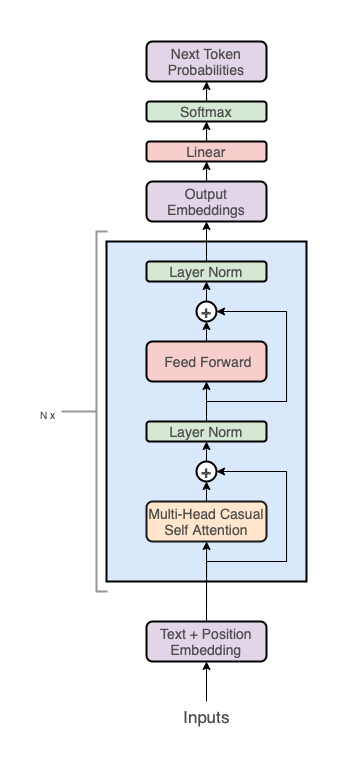
\includegraphics[height=0.8\textheight]{GPT_architecture} \\
            Image Source: \cite{mody_gpt_2023}
        \end{minipage}
        \column{0.6\textwidth}
        \begin{minipage}[c][\textheight][c]{\linewidth}
            \large
            Examples:
            \begin{itemize}
                \item GPT \cite{radford_improving_2018}
                \item GPT2 \cite{radford_language_2019}
                \item GPT3? \cite{brown_language_2020}
                \item GPT4? \cite{openai_gpt4_2023}
                \item LlaMa \cite{touvron_llama_2023}
                \item Bloom \cite{workshop_bloom_2022}
                \item OPT \cite{zhang_opt_2022}
                \item PaLM \cite{chowdhery_palm_2022}
            \end{itemize}
        \end{minipage}
    \end{columns}
\end{frame}

\subsection{CLIP}
\begin{frame}[c]{CLIP: Multimodal Embedding Spaces}
    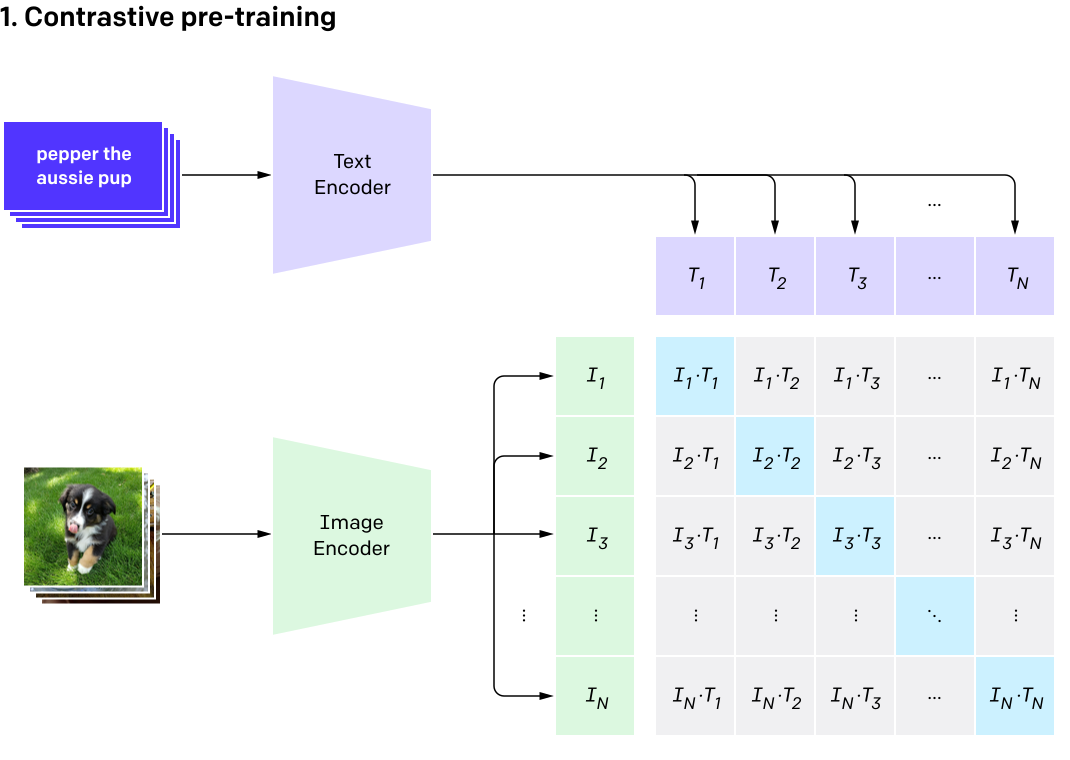
\includegraphics[height=0.8\textheight]{clip} \\
    Image Source: \cite{radford_learning_2021}
    \pnote{
        we now have an shared embedding between text and images
    }
\end{frame}

\subsection{Latent Diffusion Models}
\begin{frame}[c]{Latent Diffusion Models}
    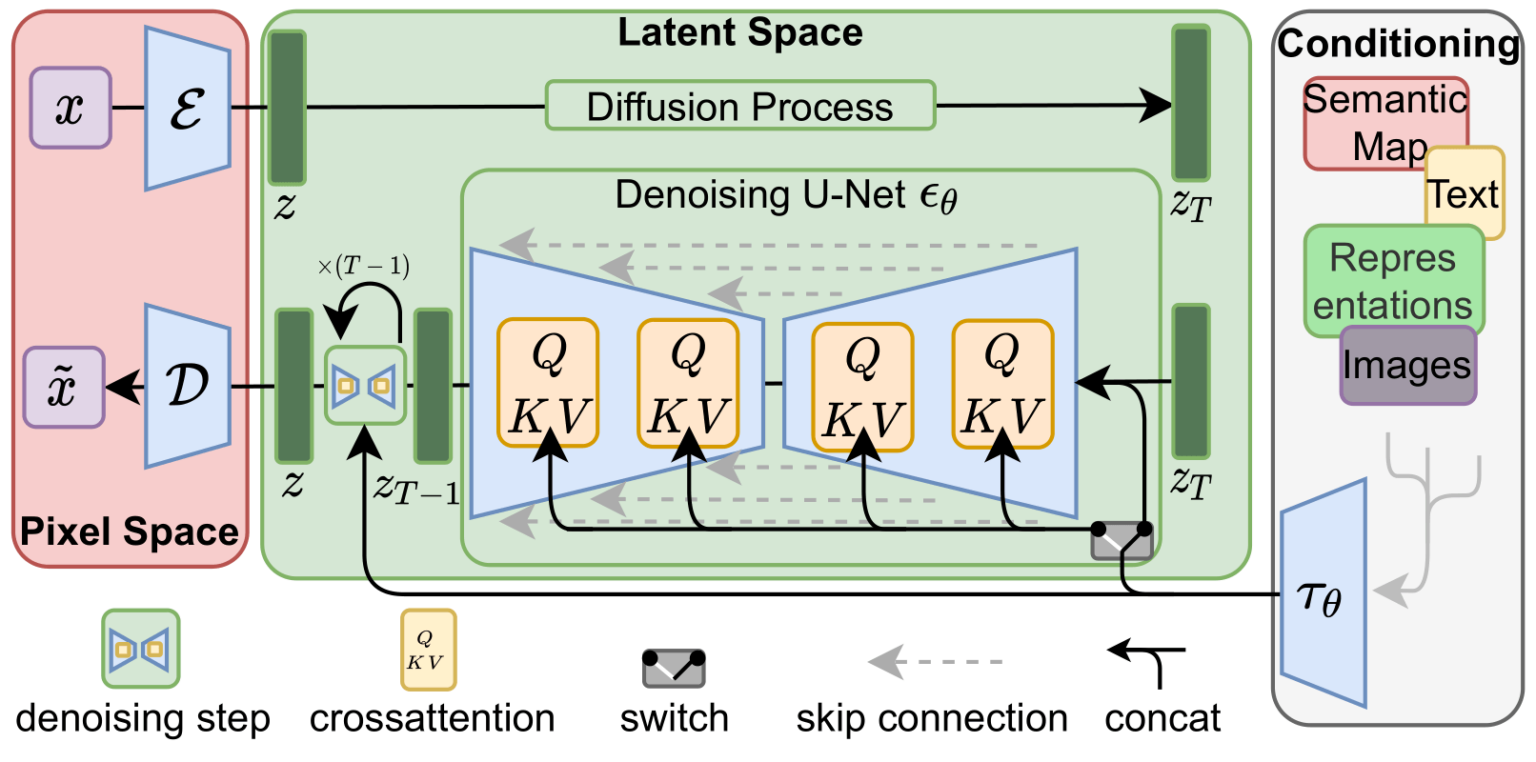
\includegraphics[width=\textwidth]{stable_diffusion} \\
    Image Source: \cite{rombach_highresolution_2022}
    % Generating images based on shared semantic embeddings
    % Diffusion \cite{sohl-dickstein_deep_2015}
\end{frame}

\subsection{Reinforcement Learning}
\begin{frame}[c]{GATO: A Generalist Agent}
    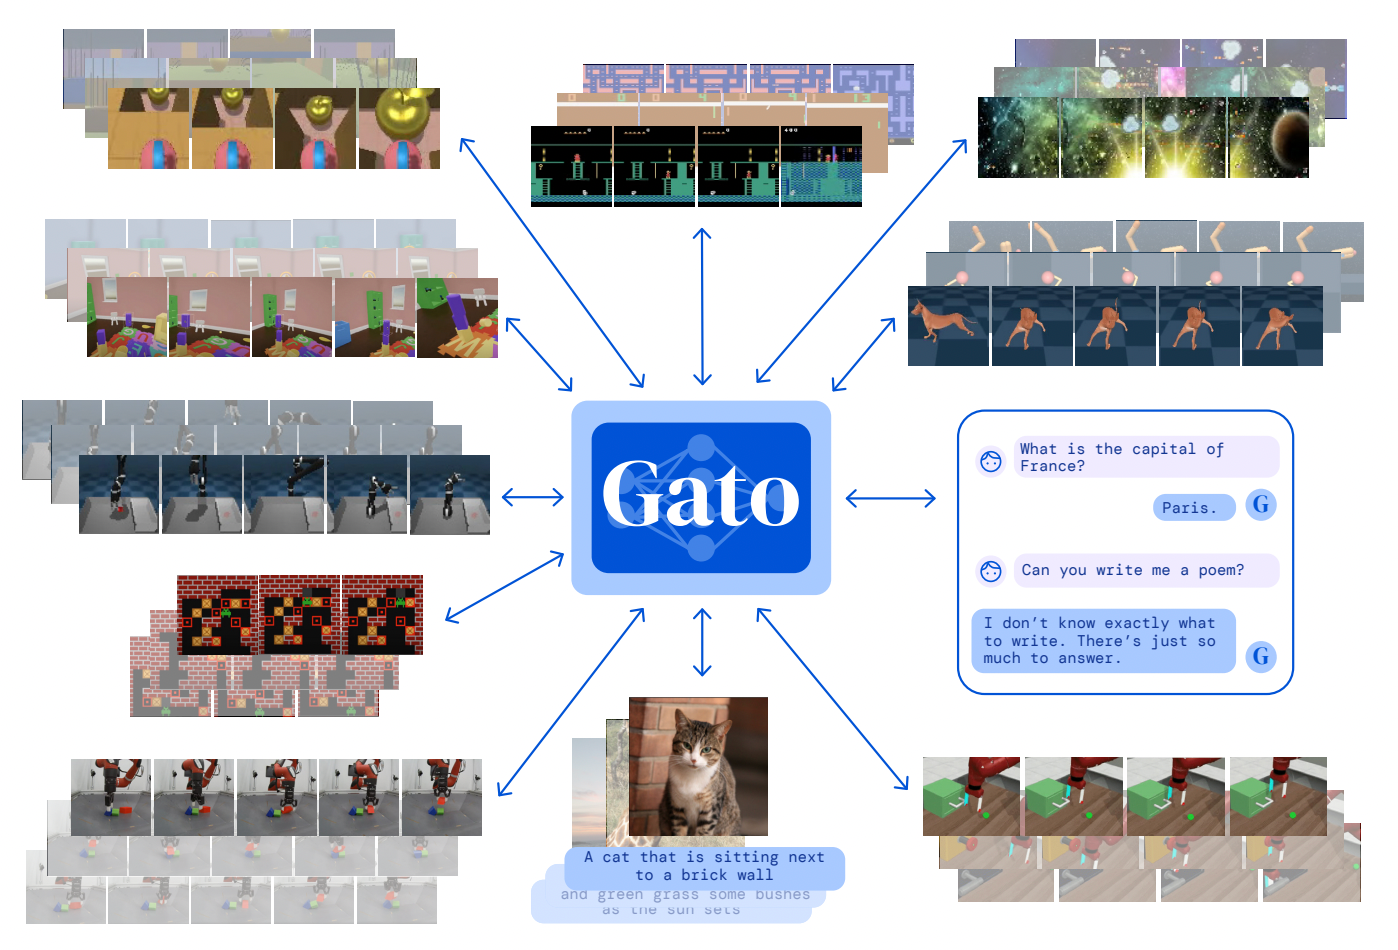
\includegraphics[height=0.8\textheight]{gato} \\
    Image Source: \cite{reed_generalist_2022}
\end{frame}

\subsection{Physics Simulation}
\begin{frame}[c]{Physics Simulation in Latent Spaces}
    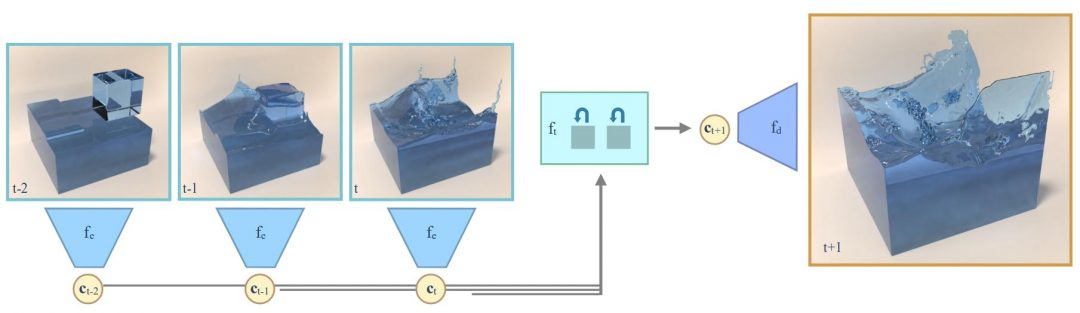
\includegraphics[height=0.8\textheight,width=\textwidth,keepaspectratio]{lsp} \\
    Image Source: \cite{wiewel_latent_2019}
    \large
    \begin{aquote}{Latent Space Physics \cite{wiewel_latent_2019}}
        ... we arrive at a data-driven solver that yields practical speed-ups, and
        at its core is more than 150x faster than a regular pressure solver.
    \end{aquote}
    \pnote{
        Speed up simulation by 150x 
    }
\end{frame}

% \subsection{Meta Cognition}
% \begin{frame}[c]{Reflexion}
%     Reflexion \cite{shinn_reflexion_2023}
%     \todo{include architecture}
% \end{frame}
